\section{Техническое задание}
\subsection{Основание для разработки}

Полное наименование системы: <<Веб-приложение \textquotedbl Социомаркет для владельцев домашних животных \textquotedbl\ >>.
Основанием для разработки программы является приказ ректора ЮЗГУ от <<24>> ноября 2023 г. №5166-с <<Об утверждении тем выпускных квалификационных работ>>.

\subsection{Цель и назначение разработки}

Веб-приложение <<Социомаркет для владельцев домашних животных>> создается с целью объединения пользователей двух групп: владельцев домашних животных и лиц, предоставляющих услуги для домашних животных. Такими лицами могут являться владельцы интернет-магазинов, предприниматели или такие же пользователи.

Задачами данной разработки являются:
\begin{itemize}
\item создание каталогов с категориями карточек на сайте;
\item Разработка клиентской части web-сайта;
\item    создание каталогов с категориями карточек на сайте;
\item    реализация формы создания и управления карточкой услуги;
\item    создание удобного поиска по каталогам карточкам;
\item    реализация взаимодействия между пользователями сайта;
\item    Разработка и развертывание инфраструктуры web-сайта и его базы данных на удаленном сервере.
\end{itemize}

\subsection{Требования пользователя к интерфейсу web-сайта}

Сайт должен включать в себя:
\begin{itemize}
    \item авторизацию;
    \item навигацию по разделам;
    \item разделение доступа к функционалу сайта для пользователя и лица предоставляющего услуги.
    \item поиск по пользователям и их товарам или услугам
\end{itemize}


\subsection{Требования к программной системе веб-приложения <<Социомаркет>>}
\subsubsection{Требования к данным программной системы}
Система должна уметь эффективно обрабатывать данные пользователей, включая личную информацию, данные о питомцах, информацию о продуктах и услугах, а также отзывы и рейтинги. Необходимо обеспечить конфиденциальность и безопасность этих данных.
На рисунке ~\ref{bd:image} представлена концептуальная модель данных программной системы в виде UML-диаграммы сущность-связь.

\begin{figure}[ht]
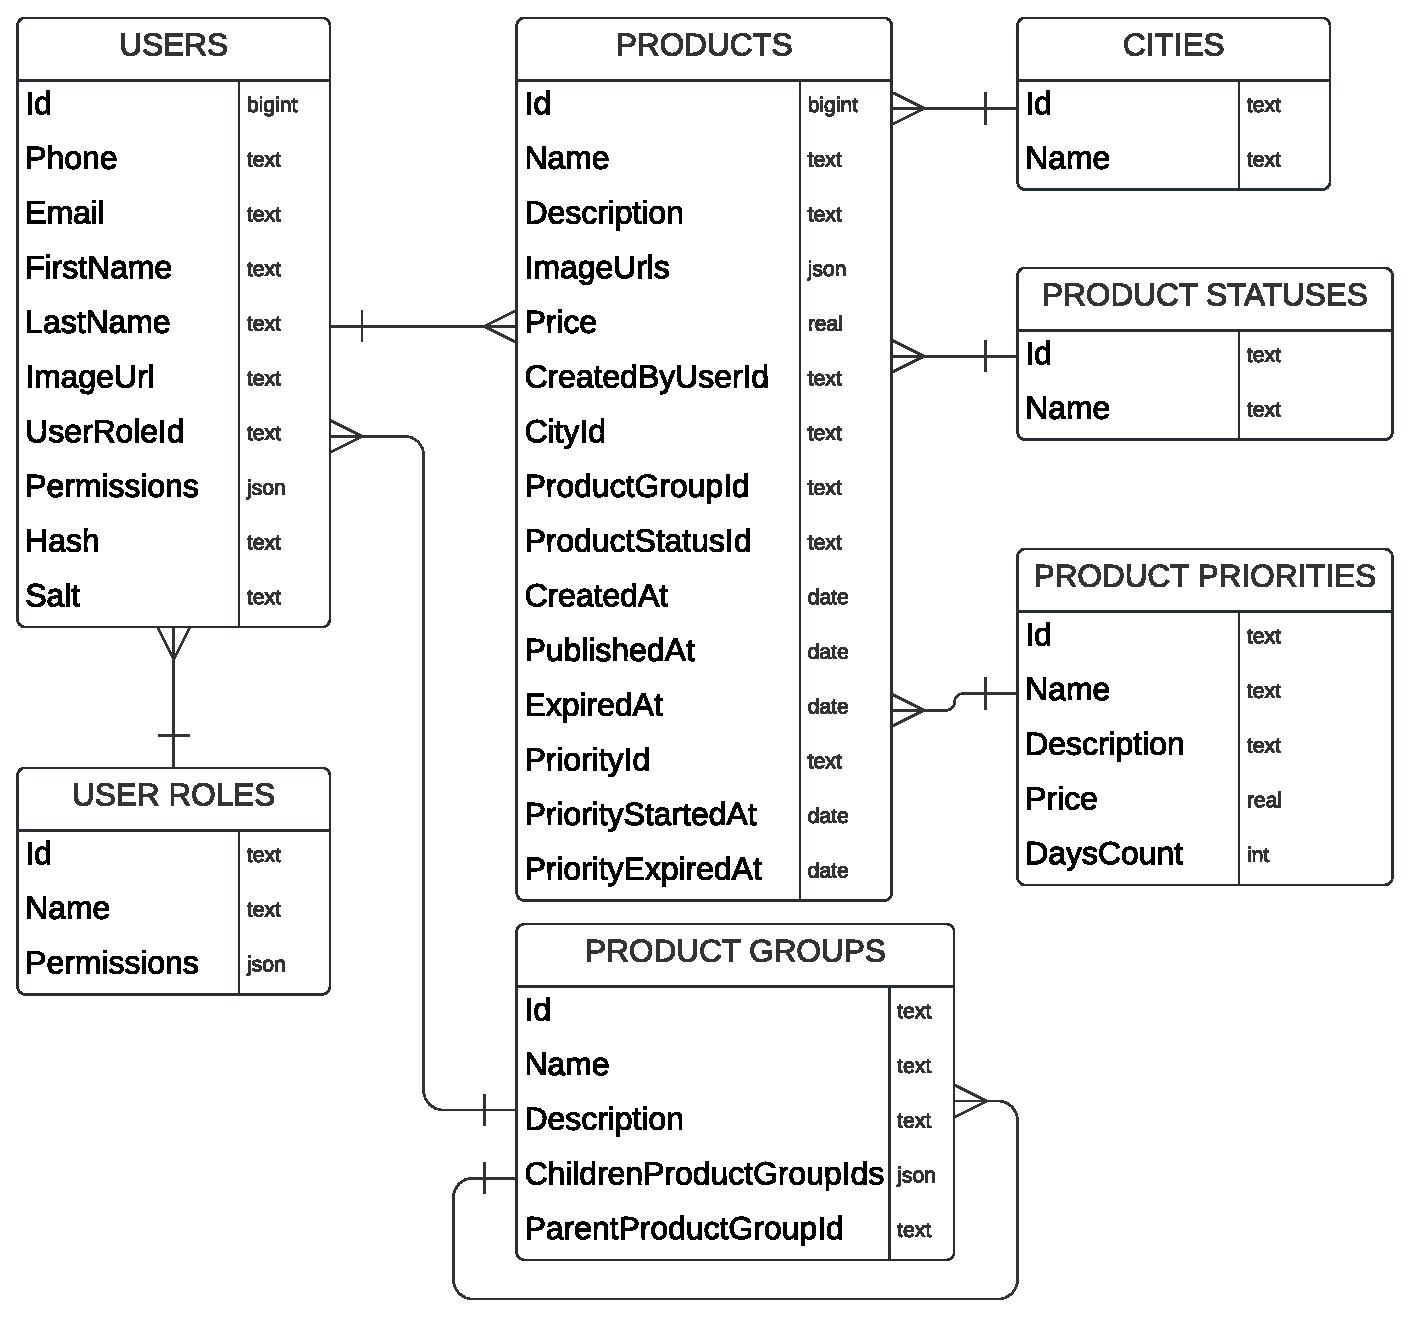
\includegraphics[width=1\linewidth]{bd}
\caption{Концептуальная модель данных}
\label{bd:image}
\end{figure}

\subsubsection{Функциональные требования к программной системе}
В разрабатываемой программно-информационной системе должно быть предусмотрено наличие двух классов пользователей: владельцев домашних животных и лиц, предоставляющих услуги или товары для них.

\subsubsection{Архитектура системы} 
Серверная часть веб-приложения <<Социомаркет>> разработана на .NET Core, обеспечивая гибкость и мощь для обработки данных. Клиентская часть, реализованная на Angular, взаимодействует с сервером через REST API. База данных построена на PostgreSQL, обеспечивая надежное хранение и быстрый доступ к данным.

\subsubsection{Вариант использования <<Авторизация пользователя>>} 
Пользователи входят в систему, используя свой логин и пароль. Предусмотрена возможность восстановления пароля через электронную почту.

\subsubsection{Вариант использования <<Авторизация лица предоставляющего услуги или товары>>} 
Поставщики услуг и товаров регистрируются в системе, предоставляя специфическую информацию о предлагаемых услугах или товарах.

\subsubsection{Вариант использования <<Поиск>>} 
Пользователи могут искать товары и услуги, используя ключевые слова и фильтры для уточнения результатов. LINQ-запросы для выполнения поисковых операций. Entity Framework Core.

\subsubsection{Вариант использования <<Просмотр каталогов карточек с товарами и услугами>>}
Пользователи могут просматривать карточки товаров и услуг в каталоге. Каждая карточка содержит информацию о товаре или услуге, включая описание, цену, фотографии и отзывы. Карточки можно фильтровать по категориям или тегам.

\subsubsection{Вариант использования <<Управление своими карточками>>}
Поставщики услуг и товаров могут создавать, редактировать и удалять свои карточки в каталоге. Это включает добавление описаний, цен, фотографий и другой релевантной информации.

\subsubsection{Вариант использования <<Инициировать обмен контактами между пользователями>>} 
Возможность отправить запрос на социальные сети другого пользователя для дальнейшего общения и сотрудничества.

\subsubsection{Вариант использования <<Редактирование профиля пользователя>>}
Пользователи могут редактировать свои личные данные, контактную информацию, а также настройки уведомлений и конфиденциальности.

\subsubsection{Вариант использования <<Просмотр профилей поставщиков услуг>>}
Пользователи могут просматривать профили поставщиков, включая описание услуг, фотографии и отзывы клиентов.

\subsubsection{Вариант использования <<Добавление отзывов и оценок>>}
После использования услуги или покупки товара пользователи могут оставлять отзывы и оценивать качество.

\subsubsection{Вариант использования <<Просмотр списка Избранное>>}
Пользователи могут сохранять понравившиеся товары или услуги в список избранных для быстрого доступа в будущем.

\subsubsection{Вариант использования <<Мобильная версия приложения>>}
Мобильная версия приложения обеспечивает удобство использования на смартфонах и планшетах, адаптируя интерфейс под мобильные устройства.


\subsection{Требования пользователя к интерфейсу приложения}
Интерфейс должен быть интуитивно понятным, удобным для пользователя, с четкой навигацией и адаптивным дизайном, подходящим для различных устройств. Желательно отказаться от диалоговых окон для крупных элементов сайта. То есть регистрация, поиск, результат поиска - все они будут на отдельных страницах, не в диалоговых окнах.
\subsection{Нефункциональные требования к программной системе}


\begin{itemize}
    \item Надёжность. Высокая стабильность и минимальное время простоя системы. Для минимизации вероятности возникновения аварийных событий серверные компоненты программной системы должны быть размещены на выделенных серверах в дата-центрах хостинг-провайдеров, прошедших сертификацию и имеющих гарантию SLA>99,8\%. Операционная системадолжна получать регулярные накопительные обновления.
    \item Безопасность. Наличие механизма проверки целостности приложения путем использования криптографических функций, основанных на подписи пакета программы. - Коммуникация с сервером по защищенному протоколу. Требования к серверу: - Регулярные обновления компонентов безопасности операционной системы. - Автоматическое обновление HTTPS-сертификатов. - Доступ к серверу должен осуществляться без разглашения IP-адреса целевой машины в целях предотвращения возможных атак типа DDoS (раcпределенный отказ в обслуживании). - Запросы к серверу должны предварительно обрабатываться на одельной машине с запущенным экземпляром сервера Nginx для контроля количества запросов и логирования обращений к серверу. - Правилами брандмауэра операционной системы основного сервера должно быть разрешено подключение к порту сервера только с IP-адреса промежуточной машины.
    \item Совместимость. Поддержка основных браузеров и операционных систем. Использование технологий адаптивной верстки frontend приложения.
    \item Аппаратные требования. Оптимизация для обеспечения производительности на различных устройствах. Предложить несколько вариантов.
\end{itemize}
